% !TEX encoding = UTF-8 Unicode
%\documentclass[twoside]{article}
\documentclass[twocolumn,10pt]{article}
\usepackage[french]{babel}
\usepackage[utf8]{inputenc}
\usepackage[T1]{fontenc}

\usepackage{amsmath}
\usepackage{amssymb}
\usepackage{amsfonts}
\usepackage{graphicx}
%\usepackage{bbm}

\usepackage[margin=2cm,top=32mm,columnsep=20pt]{geometry}
\usepackage{multirow,multicol} % Style double colonne 
\usepackage{abstract} % Customization de l'abstract 
\usepackage{fancyhdr} % en-têtes et pieds de page 
\usepackage{float} % Nécessaire pour les tables et figures dans l'environnement double colonne 

\usepackage{url}
\usepackage[colorlinks=true,linkcolor=red,urlcolor=blue,filecolor=green,citecolor=orange]{hyperref} % hyperliens 
\usepackage{dtk-logos}

\usepackage{makecell}

\usepackage[ddmmyyyy]{datetime}

\newdateformat{ddmmyyyy}{\twodigit{\THEDAY}/\twodigit{\THEMONTH}/\THEYEAR\xspace}

\def\currentyear{\the\year}
\newdate{revuedeb}{21}{04}{\currentyear}
\newdate{revuefin}{26}{04}{\currentyear}
\newdate{soutdeb}{16}{06}{\currentyear}
\newdate{soutfin}{21}{06}{\currentyear}

% En-têtes et pieds de page 
\pagestyle{fancy}  
\fancyhead{} % Blank out the default header
\fancyfoot{} % Blank out the default footer
\fancyhead[C]{Projets de SY09} % Custom header text
\fancyfoot[RO,LE]{\thepage} % Custom footer text

\setlength{\parskip}{1ex} % espace entre paragraphes 

%\renewcommand{\arraystretch}{1.5} % plus d'espace dans les tableaux 
\usepackage{booktabs} % pour de plus beaux tableaux 
\usepackage{caption} % gestion des légendes 
\captionsetup[table]{skip=10pt} % espacement recommandé 

% environnement de propriétés 
\newtheorem{propriete}{Propriété}
\newtheorem{remarque}{Remarque}

% symboles mathématiques 
\newcommand{\calN}{\mathcal{N}}
\newcommand{\bsx}{\boldsymbol{x}}
\newcommand{\bsX}{\boldsymbol{X}}
\newcommand{\bsxa}{\boldsymbol{x}_{{A}}}
\newcommand{\bsXa}{\boldsymbol{X}_{{A}}}
\newcommand{\bsxb}{\boldsymbol{x}_{{B}}}
\newcommand{\bsXb}{\boldsymbol{X}_{{B}}}
\newcommand{\bsmu}{\boldsymbol{\mu}}
\newcommand{\bsSig}{\boldsymbol{\Sigma}}
\newcommand{\bsmua}{\boldsymbol{\mu}_{{A}}}
\newcommand{\bsmub}{\boldsymbol{\mu}_{{B}}}
\newcommand{\bsSigaa}{\boldsymbol{\Sigma}_{AA}}
\newcommand{\bsSigab}{\boldsymbol{\Sigma}_{AB}}
\newcommand{\bsSigba}{\boldsymbol{\Sigma}_{BA}}
\newcommand{\bsSigbb}{\boldsymbol{\Sigma}_{BB}}
\newcommand{\transp}[1]{{#1}^\top}

% Affichage du code python 
\usepackage[cachedir=cache/minted-\jobname]{minted}
\setminted{encoding=utf8, numbersep=3pt, xleftmargin={2em}, breaklines, linenos=true}
\def\Rcode#1{\mintinline{R}{#1}}
\def\pycode#1{\mintinline{python}{#1}}
\def\latexcode#1{\mintinline{latex}{#1}}


%----------------------------------------------------------------------------------------

\title{Classification de la Santé Fœtale}

\author{Timofey Abramov, Yazan El Mahmoud, Selima Khessairi}
\date{\today}

\begin{document}

\maketitle % Insert title
\thispagestyle{fancy} % All pages have headers and footers

\begin{abstract}

Ce document constitue le rapport de projet de SY09, portant sur la classification de l'état de santé foetale, à partir du jeu de données \href{https://www.kaggle.com/datasets/andrewmvd/fetal-health-classification?select=fetal_health.csv}{Fetal Health Classification}. Ce rapport aborde l'exploration du jeu de données, puis la prédiction de l'état de santé d'un foetus grâce à des méthodes de classifications non supervisées et supervisées.

\end{abstract}


%----------------------------------------------------------------------------------------

\section*{Introduction}

La surveillance du bien-être fœtal est un enjeu majeur de santé publique. Selon l'ONU, près de 300 000 femmes décèdent chaque année de complications liées à la grossesse, principalement dans les pays à ressources limitées. La cardiotocographie (CTG), méthode largement utilisée pour monitorer la santé fœtale, permet d'évaluer le rythme cardiaque fœtal et les contractions utérines.

Cependant, l'interprétation des tracés CTG reste complexe et subjective. Une analyse plus systématique de ces données pourrait améliorer la détection précoce des situations à risque.

Pour cette raison, nous chercherons lors de cette étude à utiliser ces données afin de prédire efficacement la santé foetale.

\paragraph{Présentation du jeu de données}

Le jeu de données \href{https://www.kaggle.com/datasets/andrewmvd/fetal-health-classification?select=fetal_health.csv}{Fetal Health Classification}, rassemble 2 126 enregistrements de cardiotocographies (CTG) avec leurs caractéristiques cliniques associées. Il s'agit de données cliniques réelles collectées en milieu hospitalier. 
Il se compose de 21 variables descriptives numériques et d'une variable cible qualitative classant la santé fœtale en trois catégories : normal, suspect et pathologique.

Les variables descriptives peuvent être regroupées en trois catégories principales :
\begin{itemize}
    \item Paramètres du rythme cardiaque fœtal : valeur basale (en bpm), variabilité à court et long terme, nombre et amplitude des accélérations/décélérations
    \item Mesures utérines : nombre et durée des contractions, valeur maximale des contractions
    \item Autres indicateurs cliniques : mouvements fœtaux, activité utérine anormale, suspicion de souffrance fœtale
\end{itemize}


%----------------------------------------------------------------------------------------

\section{Analyse Exploratoire des Données}\label{sec:explor}

%-------------------------------------------------

\subsection{Visualisation de la distribution de la variable cible}\label{subsec:explor:visu}

Dans cette section, nous analysons la distribution de la variable cible, c'est-à-dire l'état de santé fœtale.

Tout d'abord, nous remarquerons que les données sont normalisées et complètes (sans valeurs manquantes). Ce qui simplifie les étapes de traitement.

\begin{figure}[H]
    \centering
    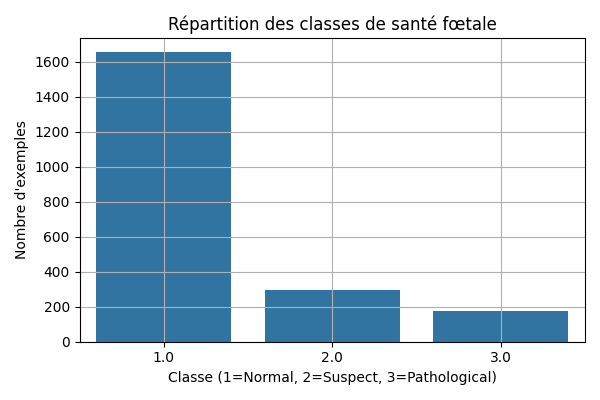
\includegraphics[width=0.45\textwidth]{projet/Distribution_maladie.png}
    \caption{Distribution de la variable cible}
    \label{fig:hist_maladie}
\end{figure}

On observe un déséquilibre marqué entre les classes, avec une surreprésentation des cas normaux: \texttt{77.84\%} des cas sont catégorisés comme "normaux", \texttt{13.87\%} des cas sont catégorisés comme "suspects" et enfin \texttt{8.27\%} des cas sont "pathologiques". Cette caractéristique devra être prise en compte dans l'analyse. 


%-------------------------------------------------

\subsection{Corréaltions entre variables}\label{subsec:explor:corr}

Les données étant toutes quantitatives (mesures de CTG) mis à part la variable cible, il est possible d'étudier leurs corrélations via une matrice de corrélation. 

L’analyse de la matrice de corrélation révèle plusieurs relations intéressantes entre les variables issues de la cardiotocographie. Certaines, comme \texttt{histogram\_mean}, \texttt{histogram\_median} et \texttt{histogram\_mode}, présentent des corrélations très fortes entre elles (supérieures à 0.9) et avec la variable \texttt{baseline\_value}, ce qui indique une forte redondance: toutes ces mesures sont liées à la fréquence et au rythme cardiaque foetaux. Concernant la variable cible \texttt{fetal\_health}, aucune caractéristique ne montre de corrélation très élevée (ce qui est courant dans les données médicales multifactorielle), mais certaines se distinguent tout de même : \texttt{prolongued\_decelerations} (0.48), \texttt{percentage\_of\_time\_with\_abnormal\_long\_term\_ variability} (0.43), et \texttt{abnormal\_short\_term\_variability} (0.47) semblent les plus informatives pour la prédiction de l’état de santé fœtale.\newline Ces résultats soulignent l’intérêt de réduire les redondances via des techniques telles que la sélection de variables ou l’analyse en composantes principales (ACP), tout en orientant les efforts de modélisation sur les variables les plus corrélées à la cible. Les variables moins corrélées, comme \texttt{fetal\_movement} ou \texttt{light\_decelerations}, pourraient s’avérer moins discriminantes mais méritent néanmoins d’être testées dans un modèle prédictif.

%-------------------------------------------------

\subsection{Analyse en Composantes Principales}\label{subsec:explor:acp}

Afin de réduire cette redondance entre variables, nous avons appliqué une ACP. Cette dernière nous a permis de visualiser les données dans un espace à 2 dimensions tout en conservant une part significative de l'information. Les deux premières composantes principales expliquent à elles seules environ 45,55\% de la variance totale.

La projection dans le premier plan factoriel montre alors une certaine séparation des classes, surtout pour les cas pathologiques et normaux, mais surtout un chevauchement entre les classes suspectes et les autres, ce qui confirme la complexité du problème.


%----------------------------------------------------------------------------------------

\section{Approches non supervisées}\label{sec:non_sup}

Afin d'évaluer la performance de différents modèles de classification sur cette tâche, nous avons tout d'abord testé une approche non supervisée à l'aide de l'algorithme k-means et la CAH, dans l'espoir de voir si les différentes classes (normal, suspect, pathologique) pouvaient émerger spontanément à partir des données.

\subsection{K-means}\label{subsec:non_sup:kmeans}

L'algorithme K-means a été appliqué sur les données brutes, avec \texttt{n\_clusters} = 3, déterminé par la méthode du coude, mais également par cohérence au jeu de données (nous avons 3 classes pour la variable). Les résultats se sont révélés insatisfaisants, avec des clusters qui ne correspondaient pas bien aux vraies classes et un indice de rand ajusté très faible (0.045). 
\begin{figure}[H]
    \centering
    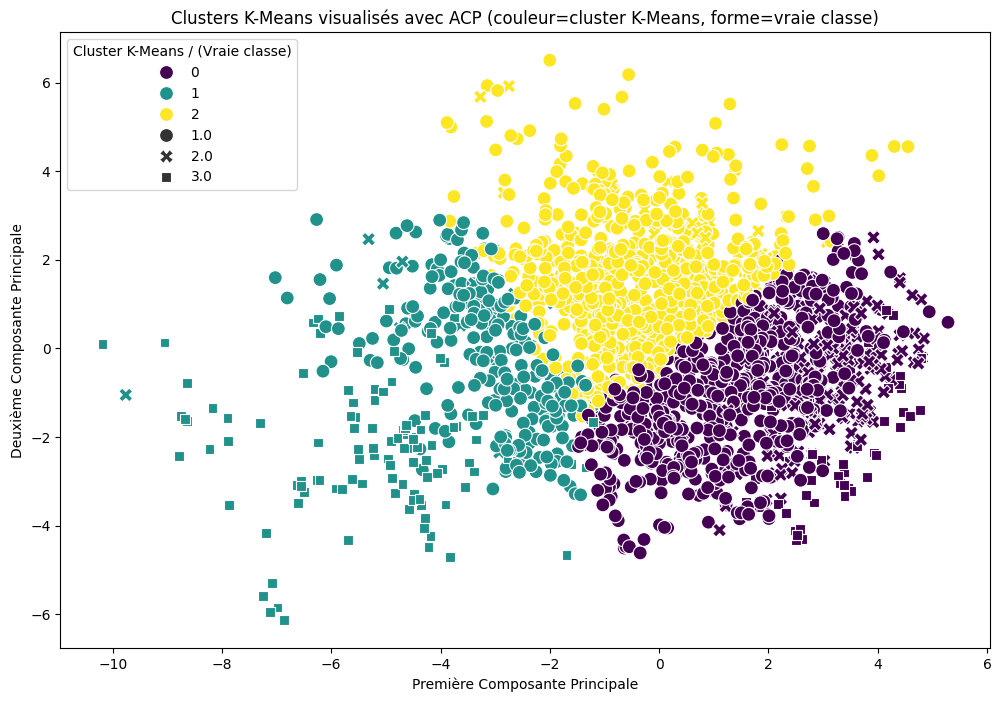
\includegraphics[width=0.45\textwidth]{projet/K_means_donnes_brutes.png}
    \caption{Comparaisons entre les classes issues des K-means et les vraies classes du jeu de données.}
    \label{fig:k_means}
\end{figure}
Ceci peut être dû à plusieurs raisons, notamment aux hypothèses fortes faites par cet algorithme. En effet, l’algorithme k-means suppose que les données forment des clusters sphériques, de taille similaire, séparés par des frontières linéaires. Or, dans notre cas, les classes ("normal", "suspect", "pathologique") se chevauchent fortement, notamment entre "normal" et "suspect", comme l’a révélé l’ACP. De plus, k-means minimise uniquement la variance intra-cluster sans tenir compte de la signification médicale des classes, qu’il ne connaît pas. Il est aussi peu adapté à des données redondantes, corrélées ou distribuées de manière non linéaire, car il repose sur la distance euclidienne. Enfin, le déséquilibre entre les classes favorise la création de clusters dominés par la classe majoritaire ("normal"), au détriment des cas plus rares mais importants comme les "pathologiques".

Afin de faire face au problème des variables redondantes, nous avons tenté d'effectuer les K-means sur les 5 premiers axes principaux d'inerties issus de l'ACP (expliquant 67\% de l'inertie) ainsi que sur les 5 variables les plus corrélées à la variable cible. Bien que nous obtenons de meilleurs résultats par rapport au K-means sur données brutes, les résultats ne sont toujours pas satifaisants (pour K-means sur ACP: ARI = 0.201 et pour les 5 variables les plus corrélées: ARI = 0.550). 
De même, l'utilisation de la distance Mahalanobis à la place de la distance euclidienne, dans le but de tenir compte de la dispersion des points qui varie selon la classe considérée (les classes ne sont pas spéhriques ni toutes pareils), n'a pas été très concluante (indice de rand ajusté de 0.189).

%-------------------------------------------------

\subsection{Classification ascendante hiérarchique (CAH)}\label{subsec:non_sup:cah}

En algorithme non supervisé, nous avons également essayé d'effectuer une CAH avec le critère de Ward, qui n'a pas non plus très bien fonctionné : en effet, le score de silhouette issu de cette dernière a été très faible (0,084), ce qui signifie que le clustering est quasiment fait aléatoirement. L'indice de Rand ajusté est également très faible (0.147). Ceci se voit également en comparant les clusters créés avec nos vraies classes issues de la variable cible.
Ceci peut être dû à plusieurs raisons: tout d’abord, les clusters sont imbriqués et non hiérarchiques. Les trois classes de \\\texttt{fetal\_health} ne sont pas nécessairement bien séparées dans l’espace des variables à cause des chevauchements entre classes ce qui nuit aux regroupements successifs de la CAH. De plus, la CAH ne gère pas bien les données bruitées ou non sphériques et ne s’adapte pas bien aux clusters de forme complexe ou allongée. Enfin, le nombre de dimensions est de nouveau problématique. En haute dimension (en l'occurence 21), la notion de distance euclidienne devient peu discriminante. Cela peut faire que les distances se ressemblent, donc les regroupements sont peu significatifs.
Afin de contourner le problème de fléau des dimensions, nous allons essayer d’appliquer la CAH sur les composantes principales issues de l’ACP, notamment les 5 premières, permettant également de supprimer la redondance issues de fortes corrélations entre certaines variables. Toutefois, même après ACP,  si les classes naturelles ne sont pas séparables linéairement, la CAH va continuer à faire des regroupements peu cohérents avec les vraies classes (\\\texttt{fetal\_health}). La CAH sur les 5 premières composantes principales n'améliore pas significativement les résultats: le score de silhouette est de 0.189 et l'indice de Rand ajusté est de 0.116.

%-------------------------------------------------

\section{Approches supervisées}\label{sec:sup}

Etant donné que nos données contiennent d'ores et déjà la variable cible (données labellisées) et que les algorithmes non supervisés n'ont pas été très concluants, nous nous intéresserons par la suite à des algorithmes supervisés. L'ensemble de ces méthodes ont été effectuées sur des données stratifiées, et divisées en données d'apprentissage (80\%) et en données de test (20\%).


%---------------------

\subsection{K Plus Proches Voisins}\label{subsec:sup:kppv}

Nous nous intéressons donc d'abord aux KPPV. Afin de déterminer le nombre optimal de voisins à choisir, une validation croisée avec 10 folds et une stratification a été effectuée. Ainsi, nous nous assurons que chaque sous-ensemble de données conserve la même distribution de classes. Le nombre optimal de voisin obtenu est k=4. Les résultats de l'application des KPPV sont présentés dans le tableau ~\ref{tab:kppv}. Nous remarquons en effet de bons résultats pour les classes \textit{normal} et \textit{pathologique} tandis que les mesures pour la classe \textit{suspects} sont plus bas. Ceci pourrait être dû à l'ambiguïté de la classe suspects, dont les mesures médicales peuvent être très similaires à celles des cas pathologiques ainsi qu'à celles des cas sains.
\begin{table}[htbp]
\begin{center}
\caption{\label{tab:kppv}Tableau résumant les mesures liées au KPPV effectué sur les trois classes}
\begin{tabular}{cccc}
\toprule
Classe & Précision & Rappel & F-1 Score \\
\midrule
Normal & 0.95 & 0.96 & 0.96 \\
Suspect & 0.69 & 0.69 & 0.69 \\
Pathologique & 0.84 & 0.77 & 0.81 \\ 
\bottomrule
\end{tabular}
\end{center}
\end{table}

Afin de limiter le problème de représentation de la classe \textit{suspect}, nous avons testé de regrouper cette dernière avec la classe pathologique (car il est toujours moins grave de diagnostiquer une maladie chez un individu sain que de ne pas le diagnostiquer alors qu'il est véritablement malade). Nous avons désormais deux classes: la classe \textit{normal} et la classe \textit{anormal}. Nous remarquons des résultats similaires au KPPV sur deux classes qui permet lui de distinguer les individus malades des individus suspects (tableau ~\ref{tab:kppv_2_classes}) notamment pour la classe \textit{anormal}. Il est ainsi plus intéressant de garder les trois classes.
\begin{table}[htbp]
\begin{center}
\caption{\label{tab:kppv_2_classes}Tableau résumant les mesures liées au KPPV effectué sur deux classes}
\begin{tabular}{cccc}
\toprule
Classe & Précision & Rappel & F-1 Score \\
\midrule
Normal & 0.94 & 0.96 & 0.95 \\
Anormal & 0.86 & 0.77 & 0.81 \\

\bottomrule
\end{tabular}
\end{center}
\end{table}

\subsection{Analyse discriminante}\label{subsec:sup:ad}

Nous avons ensuite exploré l'Analyse discriminante en testant l'Analyse Discriminante Quadratique (ADQ), l'Analyse Discriminante linéaire (ADL) et le classifieur naïf de Bayes (NB). Nous avons ainsi effectué l'hypothèse de normalité des données.
Les données ont été standardisées et stratifiées pour garantir une distribution équilibrée lors de l'entraînement et du test.


\subsubsection{Classifieur Naive Bayes Gaussien}\label{subsubsec:sup:ad:gnb}
Le modèle GNB atteint une précision globale de 81~\%. Il est particulièrement performant pour détecter les cas \textit{Normaux}, mais a des difficultés avec les cas \textit{Suspects} et \textit{Pathologiques}.

\begin{table}[htbp]
\begin{center}
\caption{\label{tab:perf}Métriques de performance par classe}
\begin{tabular}{cccc}
\toprule
Classe & Précision & Rappel & F-1 Score \\
\midrule
Normal & 0.97 & 0.85 & 0.91 \\
Suspect & 0.45 & 0.80 & 0.57 \\
Pathologique & 0.53 & 0.46 & 0.49 \\
\bottomrule
\end{tabular}
\end{center}
\end{table}

Ces résultats montrent les limites du modèle face au chevauchement entre les classes, notamment entre les cas à risque.

Cette approche permet également de prendre en compte les coûts liés aux erreurs de classification, ce qui est crucial dans un contexte médical, où certaines erreurs peuvent avoir de lourdes conséquences. La matrice des coûts utilisée est représentée dans le tableau ~\ref{tab:mat_couts}).

\begin{table}[htbp]
\centering
\caption{\label{tab:mat_couts}Matrice de coût utilisée}
\begin{tabular}{cccc}
\toprule
 & \makecell{Prédit\\Normal} 
 & \makecell{Prédit\\Suspect} 
 & \makecell{Prédit\\Pathologique} \\
\midrule
Vrai Normal & 0 & 0.5 & 2 \\
Vrai Suspect & 1 & 0 & 3 \\
Vrai Pathologique & 5 & 4 & 0 \\
\bottomrule
\end{tabular}
\end{table}


Cette approche fait baisser légèrement la précision globale à 80.3\%, mais oriente le modèle vers des décisions plus prudentes. Le modèle accepte de classer davantage de cas "Normaux" comme "Suspects" (46 contre 42 précédemment) afin de réduire le risque de sous-estimer un cas sérieux. Le rappel de la classe "Suspect" s'améliore légèrement (de 0.80 à 0.81), tandis que les performances sur la classe "Pathologique" restent stables (rappel 0.46, précision 0.53).

La nouvelle matrice de confusion montre une stratégie différente : le modèle préfère surestimer le risque (faux positifs) plutôt que de passer à côté d’un cas grave. Cela se traduit par une réduction des erreurs critiques, ce qui est bien plus adapté au domaine médical.

Même si l’accuracy globale est un peu plus basse (0.80 face à 0.92), l’approche coût-sensible est mieux adaptée à la réalité clinique. Elle permet de hiérarchiser les erreurs : mieux vaut suspecter à tort une pathologie que de la manquer. Ce compromis entre précision globale et sécurité des patients en fait une stratégie plus réaliste et responsable en médecine.

\subsubsection{Analyse discriminante Linéaire}\label{subsubsec:sup:ad:adl}

La méthode ADL suppose une distribution normale avec une matrice de covariance partagée entre les classes. Elle offre une précision globale de 85.9~\%, la meilleure obtenue jusqu’ici. La classe "Normal" est très bien reconnue, avec 93\% de précision et 95\% de rappel. Cela signifie que la quasi-totalité des cas sains sont bien identifiés.
En revanche, les performances chutent pour les classes à risque :
La classe "Suspect" n’atteint que 54\% de précision et 58\% de rappel, ce qui indique des hésitations fréquentes du modèle.
La classe "Pathologique", bien plus critique, est correctement identifiée dans seulement 46\% des cas, avec 67\% de précision.


\begin{table}[htbp]
\begin{center}
\caption{\label{tab:perf}Métriques de performance par classe}
\begin{tabular}{cccc}
\toprule
Classe & Précision & Rappel & F-1 Score \\
\midrule
Normal & 0.93 & 0.95 & 0.94 \\
Suspect & 0.54 & 0.58 & 0.56 \\
Pathologique & 0.67 & 0.46 & 0.54 \\
\bottomrule
\end{tabular}
\end{center}
\end{table}

\subsubsection{Analyse discriminante Quadratique}\label{subsubsec:sup:ad:adq}

La QDA permet une matrice de covariance différente par classe, ce qui accroît la flexibilité mais augmente significativement le nombre de paramètres à estimer.

Avec la QDA, l’objectif était d’exploiter la flexibilité accrue pour mieux séparer les classes complexes. Pourtant, ses performances globales sont légèrement en baisse, avec une précision globale de 81.2 \%.

La classe "Normal" reste bien identifiée (tableau ~\ref{tab:perf2}) et le rappel de la classe "Suspect" croît, un net progrès par rapport à la ADL. Toutefois, cette amélioration se fait au détriment de la classe "Pathologique", pour laquelle le rappel decroît fortement, bien que la précision s'améliore.

\begin{table}[htbp]
\centering
\caption{\label{tab:perf2}Métriques de performance par classe}
\begin{tabular}{cccc}
\toprule
Classe & Précision & Rappel & F-1 Score \\
\midrule
Normal & 0.95 & 0.86 & 0.90 \\
Suspect & 0.44 & 0.81 & 0.57 \\
Pathologique & 0.76 & 0.37 & 0.50 \\
\bottomrule
\end{tabular}
\end{table}

En clair, la QDA identifie mieux les cas suspects mais rate encore plus de cas pathologiques, avec 6 cas sur 35 classés à tort comme "Normaux", une erreur encore plus fréquente qu’avec la ADL.

La ADL se montre plus stable et plus adaptée à ce jeu de données. Malgré sa simplicité, elle offre un meilleur équilibre entre performance globale et sécurité. La QDA, plus complexe, échoue à mieux détecter les cas critiques, notamment les pathologies, probablement à cause de chevauchements importants entre classes. Ces résultats rappellent qu’un modèle plus complexe n’est pas toujours synonyme de meilleures performances, surtout quand il s’agit de prendre des décisions sensibles comme en médecine.

\subsection{Régression logistique}\label{subsec:sup:reg_log}
La Régression Logistique, souvent sous-estimée, est un algorithme robuste et efficace, même dans des contextes multiclasse. Nous avons utilisé ici sa version multinomiale, adaptée à notre tâche de classification en trois catégories.

Les résultats sont excellents, avec une précision globale de 88.5 \%.

La classe "Normal" est presque parfaitement reconnue, avec très peu d’erreurs critiques. La classe "Suspecte" montre des performances respectables, tandis que la classe "Pathologique", la plus critique en médecine, est détectée avec une grande précision mais encore un rappel perfectible.

\begin{table}[htbp]
\centering
\caption{\label{tab:perf}Métriques de performance par classe}
\begin{tabular}{cccc}
\toprule
Classe & Précision & Rappel & F1-score \\
\midrule
Normal & 0.94 & 0.95 & 0.94 \\
Suspect & 0.61 & 0.68 & 0.64 \\
Pathologique & 0.88 & 0.66 & 0.75 \\
\bottomrule
\end{tabular}
\end{table}

Malgré quelques confusions entre les cas "Suspect" et "Normal", la Régression Logistique se distingue par sa stabilité et sa fiabilité, notamment grâce à une quasi-absence de faux positifs critiques.

Elle parvient à classer 314 cas normaux sur 332 correctement, et 23 cas pathologiques sur 35, avec seulement 3 cas pathologiques classés à tort comme "Normaux", ce qui reste acceptable dans un cadre médical.

En résumé, la Régression Logistique combine simplicité et efficacité : elle surpasse tous les modèles précédents sauf KPPV en précision globale et offre une excellente reconnaissance des cas sains, un bon compromis pour la classe "Suspecte", et une grande prudence sur les cas pathologiques.

\subsection{Arbre de Décision}\label{subsec:sup:reg_log}
L'Arbre de Décision est un modèle très populaire, apprécié pour son interprétabilité et sa capacité à capturer des relations complexes et non linéaires dans les données. Nous l'avons appliqué à notre tâche de classification en trois catégories pour évaluer sa performance face à des modèles plus linéaires.

% Les résultats sont excellents, avec une précision globale de 90.0 \%, la plus élevée parmi les modèles testés jusqu'à présent.

La classe "Normal" est très bien reconnue, et la classe "Pathologique", la plus critique en médecine, est détectée avec un très bon rappel, supérieur à celui de la régression logistique. La classe "Suspecte", quant à elle, reste la plus difficile à cerner.

\begin{table}[htbp]
\centering
\caption{\label{tab:perf}Métriques de performance par classe}
\begin{tabular}{cccc}
\toprule
Classe & Précision & Rappel & F1-score \\
\midrule
Normal & 0.94 & 0.95 & 0.94 \\
Suspect & 0.72 & 0.64 & 0.68 \\
Pathologique & 0.81 & 0.83 & 0.82 \\
\bottomrule
\end{tabular}
\end{table}

Malgré une précision globale supérieure, l'Arbre de Décision présente un profil de risque différent. S'il identifie plus de cas pathologiques (rappel de 83 \%), il commet également plus d'erreurs critiques.

Il parvient à classer 316 cas normaux sur 332 correctement, et 29 cas pathologiques sur 35. Cependant, 5 cas pathologiques sont classés à tort comme "Normaux", ce qui représente une augmentation du risque par rapport à la régression logistique (3 cas). Cette faiblesse est un compromis direct de sa plus grande sensibilité aux cas pathologiques.




L'analyse des modèles supervisés a confirmé leur supériorité sur les approches non supervisées. Le K-Nearest Neighbors (0.906), l'Arbre de Décision (0.899) et la Régression Logistique (0.885) ont obtenu les meilleures accuracies globales (voir figure 4).


\begin{figure}[H]
    \centering
    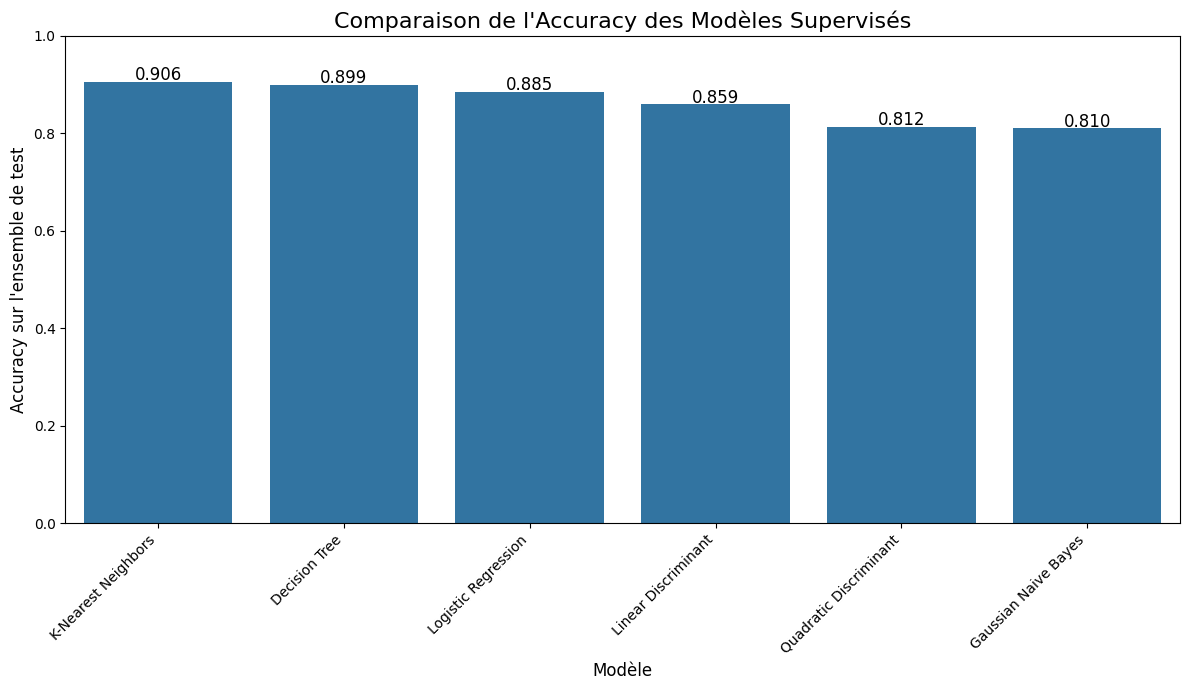
\includegraphics[width=0.45\textwidth]{projet/accuracy.png}
    \caption{Comparaison de l'Accuracy des Modèles Supervisés.}
    \label{fig:k_means}
\end{figure}

%------------------------------------------------



%------------------------------------------------

\section{Conclusion}\label{sec:sup}

En somme, ce projet a démontré que les approches supervisées sont très efficaces pour prédire la santé fœtale, surpassant largement les méthodes non supervisées qui ont échoué face à la complexité des données. Les modèles K-Plus Proches Voisins, Arbre de Décision et Régression Logistique se sont avérés les plus performants, avec des précisions globales autour de 90\%. L'analyse révèle cependant un compromis crucial : si l'Arbre de Décision détecte le plus de cas pathologiques, la Régression Logistique se montre plus fiable en minimisant les erreurs de diagnostic les plus graves, ce qui en fait un choix potentiellement plus sûr en contexte clinique. 



% Annexes

\appendix
\section{Signification médicale des variables}

\subsection{Variables Numériques}
\begin{itemize}
    \item \textbf{baseline\_value} – Rythme cardiaque fœtal de base (en bpm), normalement entre 110--160 bpm. La distribution montre une majorité de valeurs dans cette plage (fœtus sains), avec quelques cas <110 bpm. Les fœtus "à risque" présentent une médiane plus élevée et des outliers plus fréquents.

    \item \textbf{accelerations} – Nombre d’accélérations cardiaques par seconde, indicateur de bonne santé. Majoritairement nulles (histogramme), sauf pour les fœtus sains (boxplot).

    \item \textbf{fetal\_movement} – Fréquence des mouvements fœtaux par seconde. Distribution asymétrique : peu de mouvements fréquents vs absence majoritaire.

    \item \textbf{uterine\_contractions} – Fréquence des contractions utérines par seconde. Pic à 0, puis distribution normale (médiane ≈0.005). Les fœtus sains ont des contractions plus fréquentes.

    \item \textbf{light\_decelerations} – Décélérations légères liées aux contractions. Histogramme décroissant (majorité à 0).

    \item \textbf{severe\_decelerations} – Décélérations sévères (potentiellement pathologiques). Absentes dans ce jeu de données (toutes valeurs à 0).

    \item \textbf{prolongued\_decelerations} – Décélérations >2 min. Rares (quelques valeurs à 0.001--0.003), exclusivement associées aux fœtus pathologiques (boxplot).

    \item \textbf{abnormal\_short\_term\_variability} – Variabilité anormale à court terme (\%). Distribution bimodale (50--75 et 20--45). Corrélée à la pathologie (outliers bas pour les "à risque").

    \item \textbf{mean\_value\_of\_short\_term\_variability} – Moyenne de la variabilité à court terme. Pic à 1 (faible variabilité dominante). Médiane plus basse pour les pathologiques.

    \item \textbf{percentage\_of\_time\_with\_abnormal\_long\_term\_variability} – Pourcentage de temps en variabilité longue anormale. Pic à 0, mais séparation claire entre classes (boxplot).

    \item \textbf{mean\_value\_of\_long\_term\_variability} – Moyenne de la variabilité longue. Pics à 0 et 9.
\end{itemize}

\subsection{Métriques d'Histogramme (dérivées du CTG)}
\begin{itemize}
    \item \textbf{histogram\_width/min/max} – Largeur, minimum et maximum de l’histogramme des fréquences cardiaques. Largeur majoritairement entre 0--150 bpm, min souvent à 50, max centré à 150 (distribution normale).

    \item \textbf{histogram\_number\_of\_peaks/zeroes} – Nombre de pics/valeurs nulles. Peaks : 1--5 pics dominants. Zeroes : rares (pic à 0).

    \item \textbf{histogram\_mode/mean/median/variance/tendency} – Statistiques descriptives de l’histogramme. Distributions similaires pour mode, moyenne et médiane.
\end{itemize}

\vspace{0.5em}
\noindent \textit{Note} : Les métriques d'histogramme résument la distribution des fréquences cardiaques issues des cardiotocogrammes (CTG). Elles permettent une analyse diagnostique simplifiée.

\section{Analyse exploratoire des données}
\subsection{Matrice de corrélation complète}
\begin{figure}[H]
    \centering
    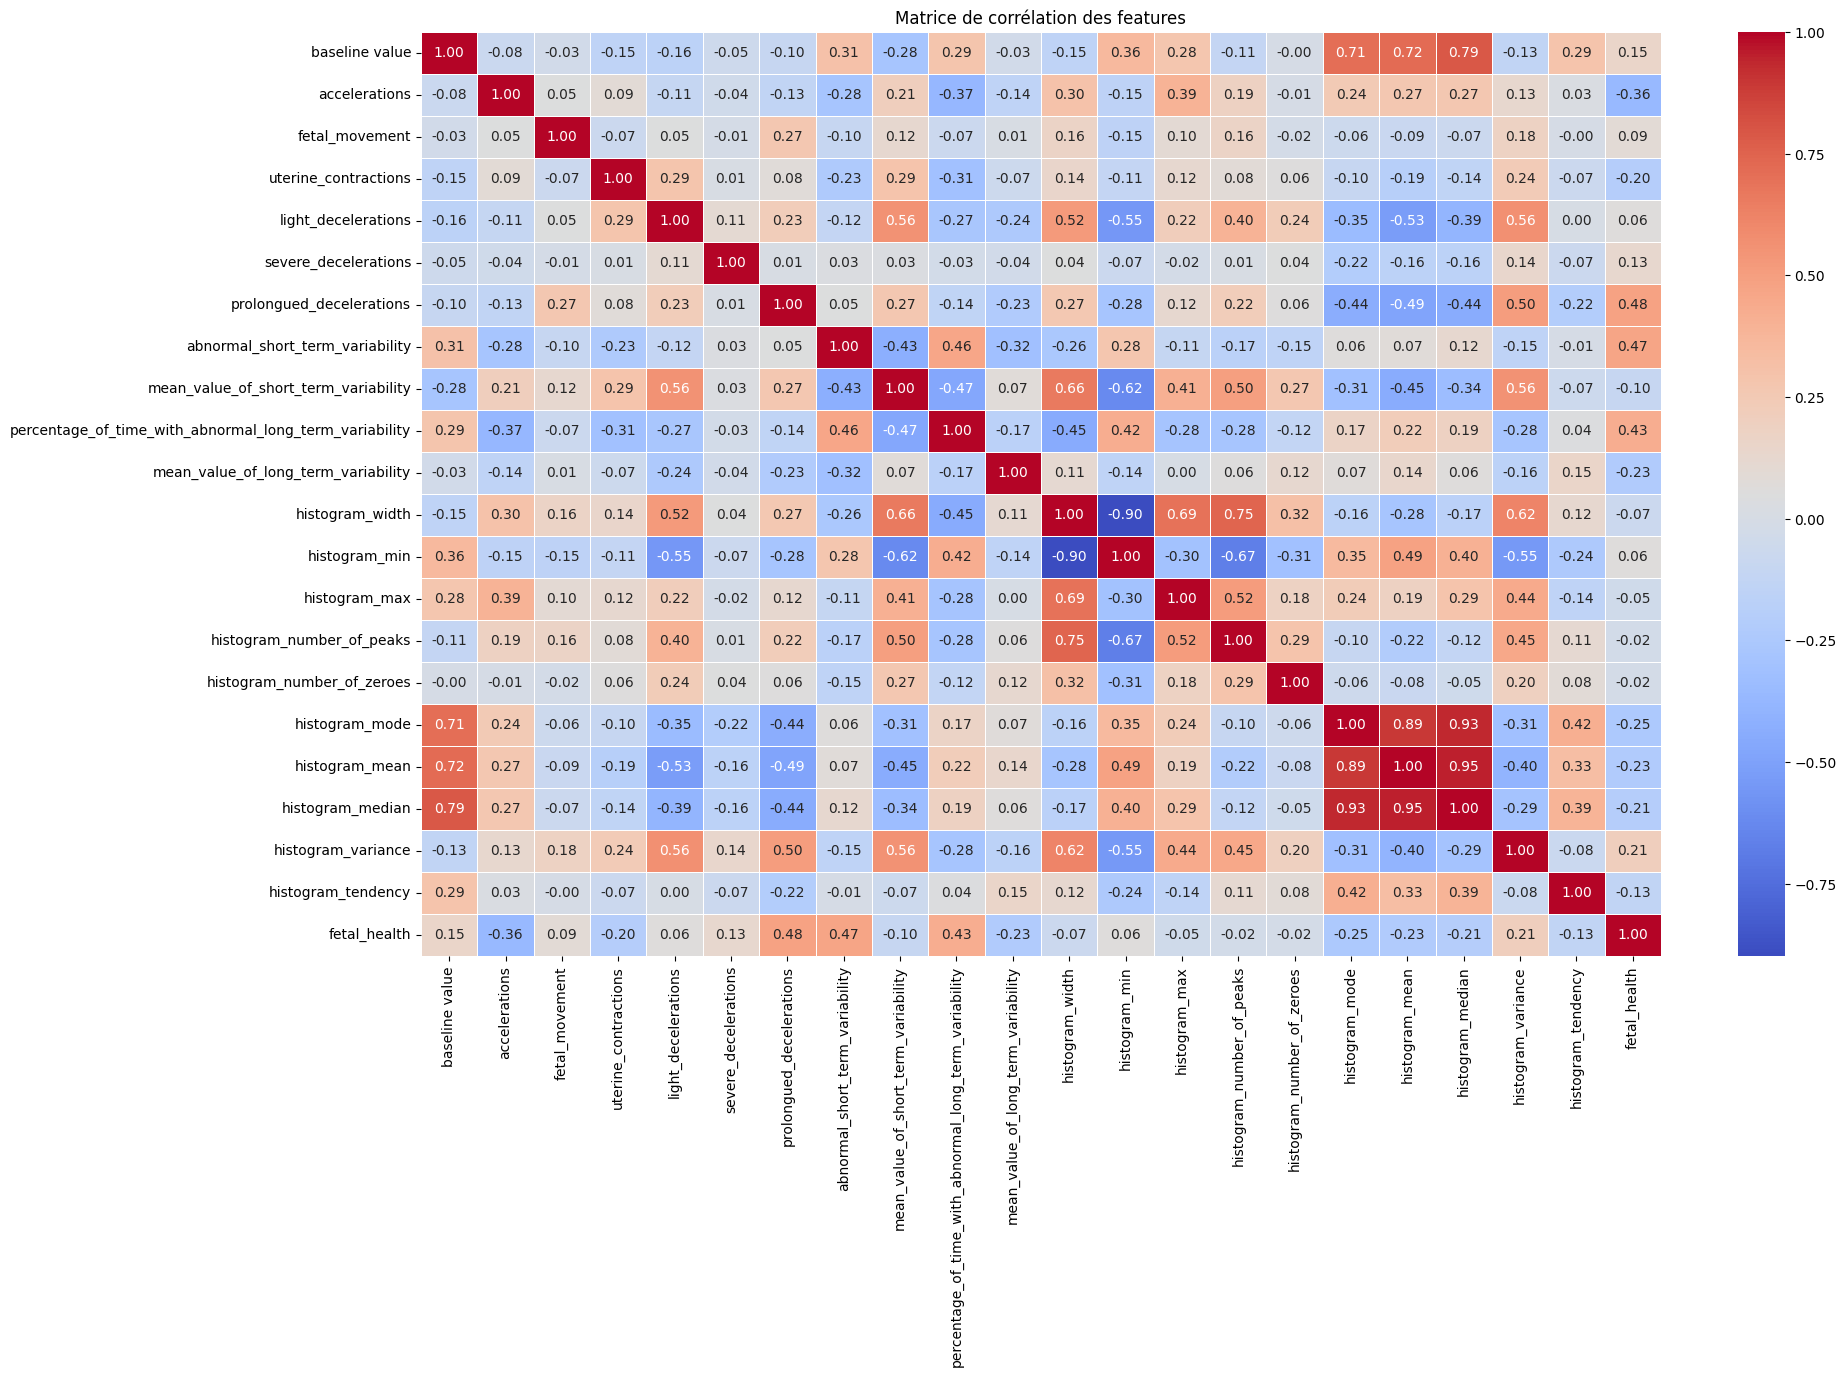
\includegraphics[width=0.45\textwidth]{matrice de corrélation_non tronquée.png}
    \caption{Matrice de corrélation des features}
    \label{fig:mat_corr}
\end{figure}

\end{document}
